\documentclass[12pt,a4paper]{article}

\usepackage[utf8]{inputenc}
\usepackage{graphicx}
\graphicspath{{data/outputs/}{xgboost_stats/}{outputs/}}
\usepackage{hyperref}
\usepackage{amsmath,amssymb}
\usepackage{booktabs}
\usepackage{caption}
\usepackage{enumitem}
\usepackage{array}
\usepackage{geometry}
\usepackage{setspace}
\usepackage{textcomp}
\usepackage{titlesec}

\geometry{margin=0.8in}
\doublespacing

\begin{document}


\begin{titlepage}
  \centering
  \vspace*{2cm}
  {\LARGE\bfseries 
  Predicting Cryptocurrency Market Bubbles Using Machine Learning\par}
  
  \vspace{1.5cm}
  {\large DSE4211 Digital Currency\par}
  {\large AY2025/26 Semester 2\par}
  \vspace{1.5cm}
  {\large
    \begin{tabular}{ll}
      Chong Yi Ting              & (A0257973L) \\
      Yan Shuhe            & (A0281964R) \\
      Cheo Chong Han       & (A0271673Y) \\
      Vivienne Tsui        & (A0266845N) \\
      Seong Yeon           & () \\
      Mulan Qin            & (A0262389R) \\
    \end{tabular}
  \par}
  \vspace{2cm}
  {\large \today\par}
\end{titlepage}

\pagenumbering{gobble}
\tableofcontents
\newpage

\pagenumbering{arabic}
\setcounter{page}{1}

%% Section 1: Introduction
\section{Introduction}
\subsection{Motivation}

Speculative bubbles are hard to detect in real time, more so in cryptocurrency markets where prices are driven by sentiment, narratives, and liquidity, rather than fundamental valuation anchors. Combined with strong retail participation and rapid information diffusion, this makes bubble occurrences more frequent and severe than in traditional asset classes. 

Major cryptocurrency crashes (eg. 2018 and 2022) have erased trillions of dollars and triggered spillovers into decentralized finance and venture capital ecosystems. However, existing methods such as the Generalized Supremum Augmented Dickey-Fuller (GSADF) test remain backward-looking and do not provide actionable early warning signals. 

This motivates a machine learning (ML) approach as modern ML models can capture complex, non-linear interactions across high-dimensional feature spaces, making them well-suited to the regime-shifting dynamics of cryptocurrency markets. By integrating market, sentiment, attention and macroeconomic features, this study aims to develop a forward-looking early warning system for next-day market states.

\subsection{Background}

Since Bitcoin's introduction in 2009, cryptocurrencies have evolved into a global asset class, reaching a peak market capitalization over \$3 trillion in 2021. However, the cryptocurrency market remains highly volatile and structurally prone to sentiment-driven price dynamics. 

A speculative bubble occurs when prices deviate persistently from fundamental value due to self-reinforcing expectations of future price increases. In cryptocurrency markets, this effect is amplified by the absence of valuation benchmarks, the dominance of retail investors and the influence of social media and algorithm-driven herding behavior. 

Bitcoin has experienced four major bubble crash cycles in 2011, 2013, 2017 and 2021. Despite differing triggers, these crashes exhibit common patterns, including rising retail attention, surging trading volumes, extreme sentiment and large deviations from historical price trends. This thus motivates a feature-engineering approach to capture the behavioral and structural signatures of bubble dynamics. 

We employ the GSADF test to identify periods of explosive price behavior and use these labels as ground truth, anchoring the ML framework in a rigorous econometric foundation. 

\subsection{Research Question}

This study addresses the following research question: 
\textit{Can machine learning models trained on market, sentiment and macroeconomic features provide reliable next-day early warning signals for cryptocurrency bubble formation and collapse?}    
To answer this, we consider two sub-questions:
\begin{enumerate}
    \item Which feature categories, technical, sentiment, macroeconomic or attention-based, contribute most to predicting bubble states?
    \item Do predictive patterns generalize across cryptocurrencies, or do asset-specific models outperform a global model?
\end{enumerate}
We evaluate three model classes of increasing complexity: a LASSO-penalized logistic regression, an XGBoost model, and a Long Short-Term Memory (LSTM) network, comparing both predictive performance and generalizability. 


%% Section 2: Lit review
\section{Literature Review}

Cryptocurrency markets present a challenge to traditional financial theory due to their high volatility, decentralized structure and vulnerability to speculative bubbles. The absence of fundamental valuation anchors and the influence of sentiment, technological development and macroeconomic conditions result in complex, non-stationary price dynamics that are difficult to model using conventional approaches. 

The GSADF procedure (Phillips et al., 2015) is a widely used econometric method for detecting bubble behavior by identifying locally explosive dynamics in price series. While effective for ex-post identification, its backward-looking nature limits its usefulness for prediction in environments driven by multiple interacting factors. 

Recent literature addresses this limitation by integrating ML techniques. Fang et al. (2022) document the growing convergence of econometric and ML approaches, showing that hybrid models outperform purely statistical methods in capturing regime shifts. 

Thomas and Natchimuthu (2025) highlight the heterogeneity of cryptocurrency bubbles across historical episodes, emphasizing the need for adaptive models. Atsiwo (2025) further demonstrates that combining econometric labelling with sentiment extraction and ensemble learning improves predictive performance. 

Building on the existing work, our study extends the literature in three ways. Firstly, we adopt a multi-asset framework across six major cryptocurrencies: BTC, ETH, BNB, ADA, SOL and DOGE. Secondly, we incorporate a comprehensive feature set spanning microstructure, sentiment, macroeconomic variables and retail attention proxies. Lastly, we introduce a three-class classification: non-bubble, bubble creation and bubble collapse, to provide more granular early warning signals.


%% Section 3: Data Prepocessing
\section{Data Preprocessing}
\subsection{Data Sources and Integration}
 
The dataset spans May 1, 2018 to Dec 31, 2024 ($T = 2437$ trading days), collected from four sources. 
\begin{itemize}
    \item \textbf{Cryptocurrency market data}: Daily OHLCV for six assets BTC, ETH, BNB, ADA, SOL, DOGE was retrieved from Binance via CCXT, yielding 13,365 observations. 
      \item \textbf{Macroeconomic indicators}: Six FRED series capture broader macroeconomic context, including Federal Funds Rate, 10Y Treasury Yield, VIX, M2 Money Supply, CPI, and 10Y Real Rate. Monthly series were forward filled to daily frequency. 
    \item \textbf{Sentiment data}: The Crypto Fear and Greed Index $F_t \in [0,100]$ from Alternative.me provides daily sentiment readings. Search interest data was collected from Google Trends to capture retail investor attention. Two categories of search terms were tracked. First, coin specific queries ($G_{c,t}$ for each $c \in \mathcal{C}$) measure asset level attention. Second, five market-wide keywords were selected based on their relevance to bubble dynamics:

\begin{table}[h]
\centering
\small
\begin{tabular}{ll}
\toprule
Keyword & Rationale \\
\midrule
``buy bitcoin'' & Purchase intent, spikes during FOMO \\
``crypto crash'' & Fear indicator, elevates near tops and corrections \\
``sell crypto'' & Exit intent, contrarian signal \\
``bitcoin price'' & General retail attention \\
``altcoin season'' & Late-stage rotation to speculative assets \\
\bottomrule
\end{tabular}
\end{table}
 
\end{itemize}
The five datasets were merged on date using outer joins. Missing values from weekend gaps in macroeconomic data and different listing dates across coins were handled via forward fill for time series and median imputation for remaining gaps after feature computation.

\subsection{Feature Engineering}
 
Features were computed independently per cryptocurrency, with each category targeting a distinct economic signal relevant to bubble dynamics. We construct features spanning seven categories: returns and price dynamics (simple and log returns, moving average ratios, price z scores), volatility (daily range, ATR, realized volatility), volume (volume ratios, price volume correlation), technical indicators (RSI, Rate of Change, price positions), sentiment measures (Fear and Greed Index, Google Trends), macroeconomic context (Fed Funds Rate, yield spread, VIX, M2 growth), and lagged and calendar features. For date-related calendar features, we apply cyclical encoding: month and day of week are each mapped to sine and cosine projections, yielding \texttt{month\_sin}, \texttt{month\_cos}, \texttt{day\_of\_week\_sin}, and \texttt{day\_of\_week\_cos}. This preserves the circular continuity of calendar periods (e.g., December adjacent to January) in a form directly usable by linear and neural models. Table~\ref{tab:feature_summary} in the Appendix summarizes the full feature set with formulas and economic rationale for including them.


\subsection{Target Variable Construction}
 
The target variable is derived from the Generalized Supremum Augmented Dickey Fuller (GSADF) test statistic, which detects explosive behavior in price series. Following Phillips et al. (2015), the GSADF statistic identifies periods where prices deviate from a random walk, characteristic of bubble formation. 
The bubble label $y_{c,t} \in \{0, 1, 2\}$ is defined as:
\begin{equation}
y_{c,t} = \begin{cases}
0 & \text{(Not Bubble)} \\
1 & \text{(Bubble Creation)} \\
2 & \text{(Bubble Collapse)}
\end{cases}
\end{equation}
Labels are computed at both 90\% critical value thresholds. To frame the task as next day prediction, labels are shifted forward by one period:
\begin{equation}
y_{c,t}^{\text{lead}} = y_{c,t+1}
\end{equation}
This ensures the model uses information available at time $t$ to predict the bubble state at $t+1$, preventing lookahead bias. 
 
\subsection{Data Standardisation}
LASSO, LSTM, and PCA require standardised data as inputs. For numerical features, we apply StandardScaler within each coin. Date-related features (month, day of week) are cyclically encoded during feature engineering as described in Section~3.2 and are not re-scaled. The final dataset summary can be seen in Table~\ref{tab:dataset_summary}. 

\subsection{Exploratory Data Analysis: Dimensionality Assessment}
We utilised PCA strictly as an exploratory diagnostic tool to assess multicollinearity. To prevent data leakage, we applied a chronological train-test split and fitted the PCA exclusively on the training set, excluding all targets. The analysis compressed our 133 engineered predictors into just 45 components while retaining 90\% of the variance. This 66.2\% dimensionality reduction mathematically confirmed the presence of severe redundant signals, directly motivating our use of LASSO feature selection (Section 4) to prevent downstream model overfitting.
 


%% Section 4 - Methology
\subsection{Evaluation Framework}
All models use the 90\% GSADF threshold as the target. To prevent look-ahead 
bias, a rolling-window scheme is used throughout. Each fold has a 9-month 
training window, a 3-month validation window for hyperparameter selection, 
and a 3-month held-out test window, stepping forward 3 months at a time. 
Over the full dataset (May 2018 to December 2024), this produces up to 22 
folds per coin.

Within each fold, LASSO and LSTM are standardised using a scaler fitted on 
the training split only. For class imbalance, LASSO and XGBoost apply SMOTE 
to the training fold, while LSTM uses manually set class weights since SMOTE 
requires independent observations and applying it to sequential data breaks 
temporal ordering and introduces leakage. Each model is tested in two 
configurations: a global model trained on all six coins with one-hot coin 
identity features, and six per-coin models trained independently.

Performance is reported using precision, recall, F1 per class, accuracy, Macro F1, and ROC-AUC. All reported results are means 
across rolling test folds.

\subsection{Models}

We evaluated three model classes of increasing complexity to answer our research questions. 

\subsubsection{Multinomial Logistic Regression Model with LASSO Penalty}

LASSO logistic regression serves as an interpretable baseline for both feature selection and prediction. The $\ell_1$ penalty shrinks coefficients of irrelevant features to zero, producing sparse models. To further address class imbalance, the model uses a one-vs-rest formulation with \texttt{class\_weight=`balanced'}, and the regularisation strength $C$ is selected by 5-fold cross-validation on the training fold itself. feature importance is evaluated by total absolute impact, which is the sum of absolute coefficient weights in classes 0, 1, 2. 



\subsubsection{XGBoost}
XGBoost captures non-linear interactions among sentiment, momentum, and macroeconomic features without requiring a predefined structure, serving as an intermediate model between the linear LASSO and sequential LSTM. Hyperparameters are tuned via randomised search optimising for Macro F1. Early stopping with a patience of 30 rounds uses the rolling-window validation split to prevent overfitting per fold. Feature importance is measured using gain.

\subsubsection{LSTM}
The LSTM network exploits sequential patterns in the time-series feature inputs to predict the next-day bubble state. Each model uses a single LSTM layer with 32 hidden units, a dropout rate of 0.30, and a 16-unit dense layer before the 3-class softmax output. Training uses the Adam optimiser (lr $= 5\times10^{-4}$, weight decay $10^{-4}$), batch size 32, and up to 15 epochs. Early stopping with patience 4 monitors validation Macro F1.

A fixed lookback of 14 days is applied uniformly across all coins and folds, balancing the capture of medium-term momentum and sentiment dynamics against training data efficiency under the rolling-window scheme. Class imbalance is addressed via inverse-frequency class weights computed from each training fold, rather than SMOTE, since synthesising arbitrary 3-dimensional sequence windows is ill-defined. For the global model, sequences are built independently per coin within each fold and then concatenated, preventing the model from learning spurious patterns across coin boundaries.




%%% Section 5 - Analysis
\section{Discussion and Analysis of the Results and Findings}

%%%%% LASSO LR Evaluation
\subsection{Evaluation of LASSO Model}
\subsubsection{Global LASSO Model}
We examine feature selection by the average of features kept in each rolling window, and find that an average of 5.53 features were kept and  133.47 were dropped. This confirms the presence of multicollinearity among features. Section 5.4 further discusses feature importance of the model. 

From Table~\ref{tab:model_comparison}, the global LASSO model achieved a macro F1 score of 0.3294, weighted F1 of 0.6063 on the test set. At the class level, the model performs very well with predicting “Not Bubble” (F1 0.6514), moderately well for “Bubble Creation” (F1 0.1541), and struggles for “Bubble Collapse” (F1 0.0279), despite the application of SMOTE on training set in each rolling window.  

\subsubsection{Per-Coin LASSO Models}
Similarly, the per-coin LASSO models also eliminate majority of the features and keep on average 4 to 5 features across all training windows. 

From Table~\ref{tab:model_comparison}, among the 6 per-coin LASSO models, the mean Macro F1 is 0.4673 and mean Weighted F1 is 0.6593, which are better than the global LASSO model. This is driven by an improvement in predicting bubble creation (F1 0.1892) and especially in bubble collapse (F1 0.0647), whereas it is not as good in predicting not bubble (F1 0.5879) compared to the global LASSO model.


%%% XGBoost Evaluation
\subsection{Evaluation of the XGBoost Model}

\subsubsection{Global XGBoost Model}

Under the rolling-window scheme, the global XGBoost model achieves a Macro F1 of 0.4275 and Weighted F1 of 0.6522 (Table~\ref{tab:model_comparison}). Performance is highly imbalanced: F1 is strong for “Not Bubble” (0.7129) but much weaker for “Bubble Creation” (0.1616) and “Bubble Collapse” (0.0951). Despite the application of SMOTE, the model remains biased toward the majority class, as minority-class signals are weak and temporally inconsistent, causing it to default to predicting "Not Bubble", which inflates aggregate metrics while limiting early-warning usefulness.Feature importance is also dominated by temporal indicators (e.g., calendar dummies), momentum variables such as \texttt{roc\_30}, and macro features like \texttt{vix\_regime} (Figure~\ref{fig:mean_features}). While these capture broad regimes, they fail to produce stable cross-asset signals for rare events.


\subsubsection{Per-Coin XGBoost Models}

Per-coin models improve upon the global model, achieving a Macro F1 of 0.4861 and Weighted F1 of 0.6348 (Table~\ref{tab:model_comparison}). Class-level F1 scores rise to 0.5622 (Not Bubble), 0.1913 (Creation), and 0.0854 (Collapse) (Table~\ref{tab:model_comparison}). Although these gains are modest, they demonstrate that asset-specific modelling recovers signals that are diluted in the pooled setting. This improvement reflects heterogeneity across cryptocurrencies: sentiment-driven assets such as DOGE and ADA align more closely with attention-based features, BTC benefits from its longer and richer bubble history, and BNB remains difficult to model due to missing exchange-specific drivers such as token burns and listing events.
 

\subsubsection{Global vs Per-Coin Comparison}

The Macro F1 gap (0.4861 vs 0.4275) highlights a fundamental trade-off between \textit{data volume} and \textit{signal consistency}. While the global model benefits from a larger training set, cross-asset heterogeneity forces it to learn an averaged decision boundary that poorly represents any individual coin. Since Macro F1 weights all classes equally, weak minority-class detection across assets penalises the global model disproportionately. Per-coin models, trained on more homogeneous data, better capture asset-specific dynamics, improving "Bubble Creation" F1 from 0.1616 to 0.1913. However, "Bubble Collapse" detection declines slightly from 0.0951 to 0.0854, suggesting that collapse signals may in fact benefit from cross-asset pooling. The higher "Not Bubble" F1 of the global model (0.7129 vs 0.5622) further confirms that pooling primarily reinforces the majority class rather than improving rare-event detection. Pooling also interacts adversely with class imbalance: heterogeneous bubble episodes across assets reduce signal coherence, making minority-class patterns harder to learn consistently. Overall, increased data volume does not offset the costs of cross-asset heterogeneity, and the Macro F1 gap reflects fundamentally asset-specific bubble dynamics. Global models may therefore appear stable in aggregate but systematically underperform in detecting the regime shifts that matter most.

  
%%%%% LSTM Evaluation
\subsection{Evaluation of the LSTM Model}

We report held-out chronological test-set precision, recall, and F1 for the three classes, using Macro F1 as the main aggregate metric because it assigns equal weight to rare event classes. Since the LSTM is implemented only as a per-coin model, evaluation focuses on six coin-specific models.

\subsubsection{Per-Coin LSTM Models}

The per-coin LSTM results, reported in Table~\ref{tab:lstm_per_coin}, show substantial heterogeneity across cryptocurrencies. Validation tuning selected thresholds of 0.35 for ADA and ETH, 0.30 for BNB, and 0.25 for BTC, DOGE, and SOL, indicating that the collapse decision boundary is asset-specific rather than shared across coins. Macro F1 ranges from 0.2428 for BNB to 0.7005 for ADA, indicating that sequential predictability differs markedly by asset. ADA achieves the strongest and most balanced performance, with high F1 scores across all three classes, including a Bubble Collapse F1 of 0.6964. BTC and DOGE also perform relatively well, with Macro F1 scores above 0.5, driven mainly by stronger detection of Bubble Creation events. By contrast, BNB and ETH perform substantially worse, with very low event-class F1 scores and weak collapse detection. SOL occupies an intermediate position: although its Not Bubble F1 is low, it still achieves moderate performance on both Bubble Creation and Bubble Collapse. 

\subsubsection{Evaluation}

Overall, the LSTM results provide mixed but meaningful evidence on the value of sequential modelling for cryptocurrency bubble prediction. On the positive side, the model appears more effective at detecting Bubble Creation than Bubble Collapse. Creation F1 exceeds 0.49 for ADA, BTC, DOGE, and SOL, suggesting that bubble formation is often preceded by gradual and learnable temporal patterns in momentum, sentiment, and macroeconomic conditions. In contrast, Bubble Collapse remains much harder to predict reliably: except for ADA, Collapse F1 remains below 0.24 for all coins. This asymmetry suggests that collapse episodes are either rarer, more abrupt, or more strongly driven by exogenous shocks that are not fully captured by historical tabular features.

The class-level results also reveal a precision–recall tradeoff in collapse detection, even after manual coin-specific class weighting, with the strongest collapse up-weighting assigned to BNB and ETH due to especially sparse collapse sequences. For several coins, the model improves sensitivity to potential collapses only at the cost of more false positives, while in other cases minority event classes are absorbed into the dominant “Not Bubble” class. This pattern is consistent with the severe imbalance of the label distribution and highlights the difficulty of learning stable collapse signals under realistic chronological evaluation. Taken together, the results suggest that LSTM can exploit temporal dependence in cryptocurrency bubble dynamics, but its predictive gains are highly coin-specific and concentrated more in bubble formation than in bubble collapse.


%% Cross Model Comparison
\subsection{Cross-Model Comparison}

Table~\ref{tab:model_comparison} reports mean Macro F1 and class-level F1 scores for LASSO, XGBoost, and LSTM, averaged across all rolling test folds at the 90\% GSADF threshold. 

\begin{table}[h]
\centering
\small
\caption{Rolling-Window Mean Metrics: LASSO vs XGBoost vs LSTM (90\% GSADF)}
\label{tab:model_comparison}
\begin{tabular}{llccccccc}
\toprule
Model & Scope & Macro F1 & Weighted F1 & Accuracy & F1 Not Bubble & F1 Creation & F1 Collapse \\
\midrule
XGBoost & Per-Coin & 0.4861 & 0.6348 & 0.6419 & 0.5622 & 0.1913 & 0.0854 \\
LASSO   & Per-Coin & 0.4673 & 0.6593 & 0.6588 & 0.5879 & 0.1892 & 0.0647 \\
XGBoost & Global   & 0.4275 & 0.6522 & 0.6654 & 0.7129 & 0.1616 & 0.0951 \\
LSTM    & Global   & 0.3862 & 0.6882 & 0.6842 & 0.7124 & 0.1826 & 0.0615 \\
LSTM    & Per-Coin & 0.3404 & 0.4818 & 0.4902 & 0.4187 & 0.1227 & 0.0998 \\
LASSO   & Global   & 0.3294 & 0.6063 & 0.6145 & 0.6514 & 0.1541 & 0.0279 \\
\bottomrule
\end{tabular}
\end{table}

\begin{figure}[h]
    \centering
    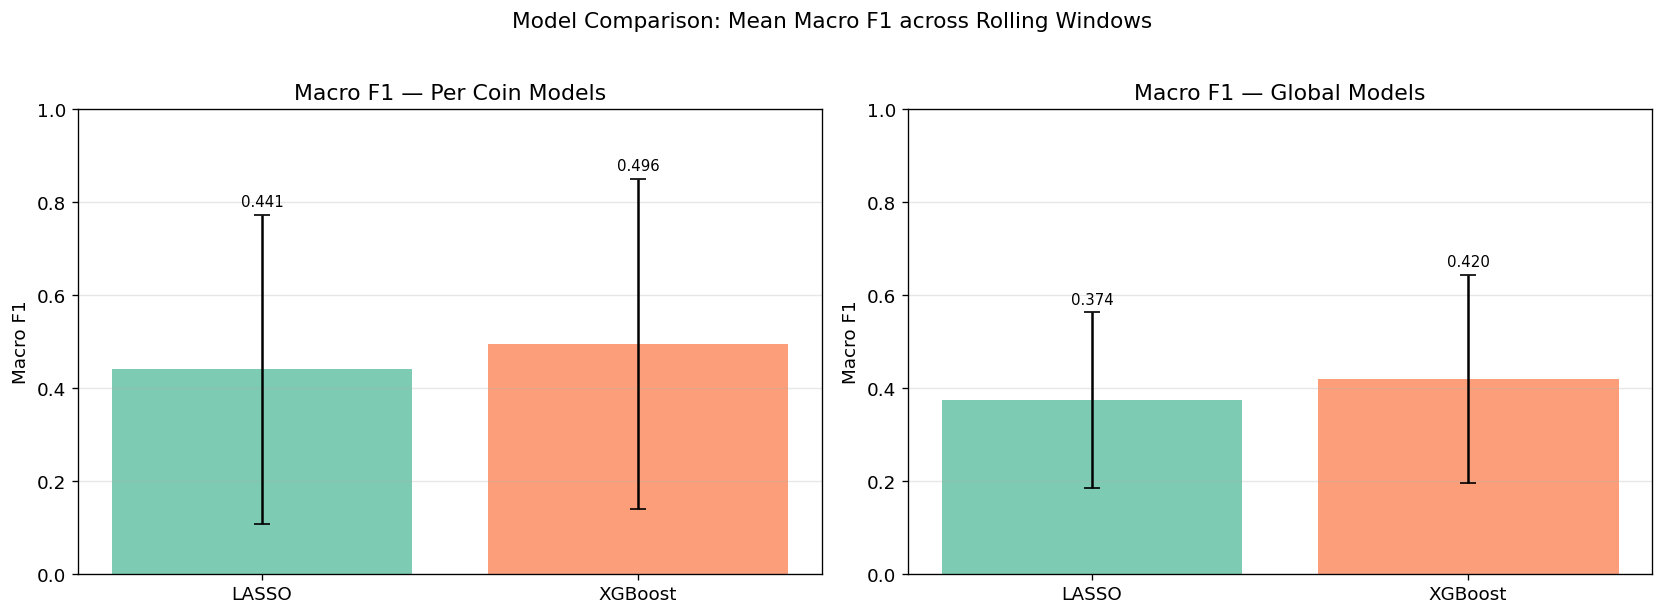
\includegraphics[width=0.9\linewidth]{macro_f1_comparison.png}
    \caption{Mean Macro F1 across rolling test folds: LASSO, XGBoost, and LSTM, per-coin and global}
    \label{fig:rolling_macro_f1}
\end{figure}

\begin{figure}[h]
    \centering
    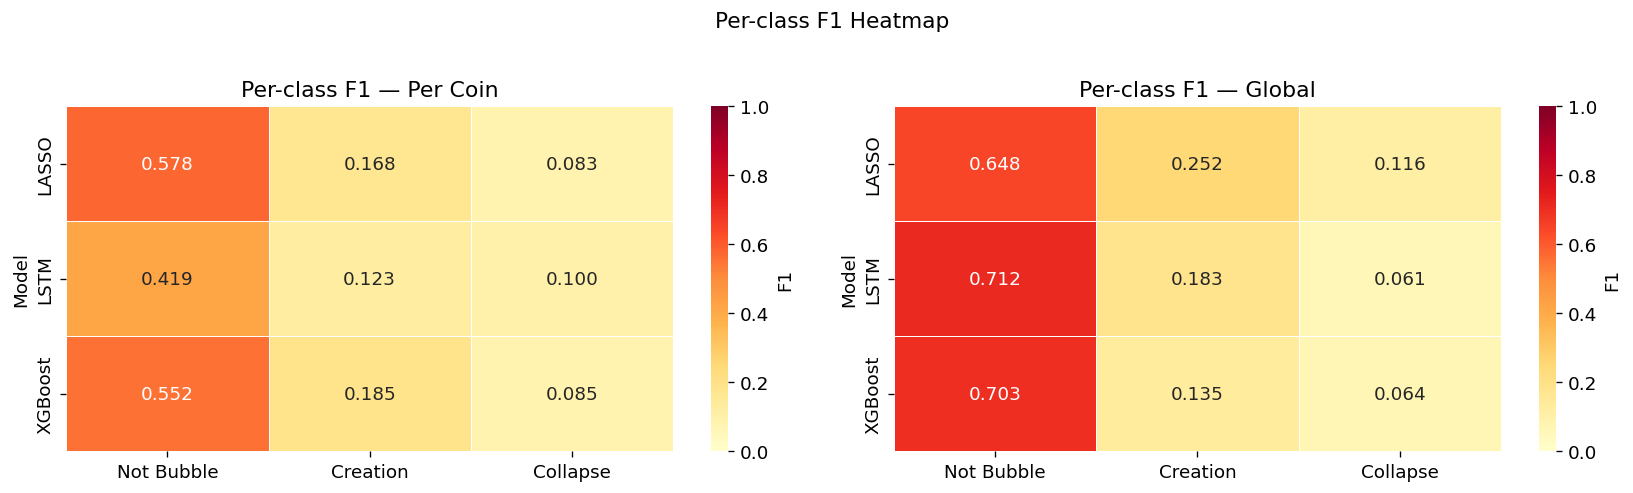
\includegraphics[width=0.9\linewidth]{per_class_f1_heatmap.png}
    \caption{Per-class F1 heatmap (Not Bubble, Creation, Collapse) averaged across rolling folds}
    \label{fig:rolling_class_f1}
\end{figure}

XGBoost per-coin leads all variants with a Macro F1 of 0.486, followed by LASSO per-coin (0.467), XGBoost global (0.428), LSTM global (0.386), LSTM per-coin (0.340), and LASSO global (0.329). For LASSO and XGBoost, per-coin variants outperform their global counterparts. LSTM reverses this: the global model exceeds per-coin by 0.046 Macro F1, suggesting it needs the larger pooled training set to learn temporal patterns effectively.

Rare event detection remains poor across all models. Collapse F1 ranges from 0.028 to 0.100 and Creation F1 from 0.123 to 0.191, with no model family standing out. Global models score higher on Not Bubble F1 (0.651 to 0.713) than per-coin variants (0.419 to 0.588), as pooling reinforces the dominant class. LSTM global achieves the highest Weighted F1 at 0.688, reflecting stronger calibration on the majority class.

%% Feature Importance
\subsection{Feature Importance}

\begin{figure}[h]
    \centering
    \includegraphics[width=0.8\textwidth]{mean_features.png} 
    \caption{Top 10 Mean Feature Importances}
    \label{fig:mean_features}
\end{figure}

Figure ~\ref{fig:mean_features} shows the top 10 most important features across training windows in LASSO global, LASSO per-coin, XGBoost global, and XGBoost per-coin models respectively. 

Across these 4 models, majority of the features are derived technical indicators from volume and price, for example, moving averages, rsi, roc. Sentiment indicators like fear \& greed index, own coin Google trend index as well buy and sell crypto Google trend index make up some of the top features too. Notably, we observe that quarter, month, and week variables contribute 4 out of 10 top features in LASSO per-coin model. Macroeconomic indicators also do not seem to be significant predictors, since only LASSO global model contains the fed funds 7 day change as the 10th most significant predictor. 

\subsection{Critical Discussion}


\subsubsection{Why Some Coins Are More Predictable Than Others}

Predictive performance varies systematically across assets: BTC and ADA sit at the top, while BNB is consistently at the bottom. This reflects an alignment problem between our feature set and each coin's dominant price-formation mechanism. BTC has the longest bubble history and is the benchmark around which our sentiment and attention features are built, while ADA's community and sentiment-driven behaviour aligns closely with Google Trends and Fear \& Greed signals. BNB by contrast is driven by Binance-specific events like token burns, listing decisions, exchange-level regulatory actions, none of which are in our features, so the model can only detect BNB bubbles when they coincide with broader episodes. ETH's utility-linked demand (gas, staking, DeFi collateral) and SOL's shorter, outage-affected history further blur their signals. The practical implication is that such a system will be selectively reliable: most trustworthy for assets with broadly-driven dynamics, least trustworthy for those with idiosyncratic or utility-linked drivers.

\subsubsection{The Asymmetry Between Predicting Creation and Collapse}

Across all models, Bubble Creation is measurably easier to predict than Bubble Collapse. This asymmetry matters more than aggregate Macro F1 suggests. Creation signals support low-cost risk reduction, but collapse signals are what determine whether an investor actually exits before drawdowns materialize, and missed exits are the costliest errors in crypto portfolios. A confident ``no collapse detected'' output also risks being read as an all-clear when it is really a blind spot. Collapse events are rare, frequently triggered by exogenous shocks such as regulatory actions or liquidation cascades, and often occur intraday rather than at the daily horizon our features resolve. Practical deployment would therefore need to pair these models with collapse-oriented signals they are not designed to capture, such as volatility-regime indicators, on-chain liquidation stress, derivatives funding flips, or intraday order-book imbalances.

%%% Section 6 - Limitations and Future Work
\section{Limitations and Future Work}

\subsection{LASSO}
The multinomial logistic regression model with LASSO penalty assumes linear relationship between bubble labels and features, whereas in reality relationships may be non-linear and more complex. A possible improvement is incorporating interaction terms in this model.
Also, as a baseline model, SMOTE is not applied to the dataset, which may weaken the predictive power for “Bubble Creation” and “Bubble Collapse”. To improve, either SMOTE or cost-sensitive learning (for instance, higher penalty weights to misclassified “Bubble Collapse”) could be applied to this model.

\subsection{XGBoost}
XGBoost, being a discriminative model that learns decision boundaries based on feature splits, may lack the structural inductive bias required to recognize the self-reinforcing, reflexive feedback loops characteristic of genuine bubbles. As a result, the models were unable to achieve a macro F1 score above 0.5. Future work could include working with different detection thresholds for what we accept as a market bubble creation or the market bubble collapsing, to tradeoff precision for better recall in model performance. 

\subsection{LSTM}
The LSTM is evaluated on a single chronological split rather than rolling windows (as used for LASSO and XGBoost), meaning cross-model comparisons should be interpreted cautiously. Although the LSTM is designed to capture temporal dependencies, its performance remains constrained by the rarity of bubble-event sequences, especially for “Bubble Collapse”. In addition, the current LSTM relies on a fixed lookback window and historical tabular features, which may not fully capture abrupt exogenous shocks such as regulatory announcements or sudden shifts in market sentiment. Future work could extend the feature set with news-based sentiment, social media signals, and on-chain indicators, and compare the current LSTM with more flexible sequence architectures such as attention-based models or Transformers.



%%% Section 7 - Conclusion 
\section{Final Conclusion}

This study examined whether machine learning models trained on market, sentiment, attention, and macroeconomic features can provide next-day early warning signals for cryptocurrency bubble formation and collapse. Overall, the results suggest that such signals do exist, but their predictive strength is uneven across bubble states and across assets. In particular, Bubble Creation appears more predictable than Bubble Collapse, implying that the build-up to speculative bubbles contains more gradual and learnable patterns, whereas collapse events are rarer, more abrupt, and therefore harder to forecast reliably.

Our findings also indicate that early warning patterns are not fully generalizable across cryptocurrencies. Model performance varies substantially by coin, suggesting that bubble dynamics remain strongly asset-specific rather than governed by a single transferable structure. Taken together, the results provide partial support for our research question: machine learning can offer useful early warning signals for cryptocurrency bubble regimes, especially for bubble formation, but predicting bubble collapse remains a fundamentally more difficult task.



%%% Section 8 - References
\newpage
\section{Appendix}

\subsection{References}
1. Fang, F., Ventre, C., Basios, M. et al. (7 February 2022) Cryptocurrency trading: a comprehensive survey. Financ Innov 8, 13 \url{https://doi.org/10.1186/s40854-021-00321-6} 

2. Thomas, Nidhiya \& Natchimuthu, Natchimuthu. (2025). Bubble dynamics: Understanding the development trajectory of the cryptocurrency market through its bubble periods. Multidisciplinary Reviews. \url{https://www.researchgate.net/publication/396171490_Bubble_dynamics_Understanding_the_development_trajectory_of_the_cryptocurrency_market_through_its_bubble_periods} 

3. Atsiwo, Abraham. (2025). A three-step machine learning approach to predict market bubbles with financial news. \url{https://www.researchgate.net/publication/396715441_A_three-step_machine_learning_approach_to_predict_market_bubbles_with_financial_news} 





\newpage
\subsection{Rebuttal and Changes made}



\subsection{Tables and Figures}


\begin{table}[h]
\centering
\small
\caption{Final dataset summary after preprocessing}
\label{tab:dataset_summary}
\begin{tabular}{lrl}
\toprule
Attribute & Value & Notes \\
\midrule
Date range & 2018-05-01 to 2024-12-31 & After lead shift \\
Total observations & 13,359 & 6 dropped from lead \\
Cryptocurrencies & 6 & BTC, ETH, BNB, ADA, SOL, DOGE \\
Features & 133 (per-coin models), 139 (global models) &  +6 coin dummies for global models \\
Target classes & 3 & Not Bubble, Creation, Collapse \\
\bottomrule
\end{tabular}
\end{table}




\begin{table}[h]
\centering
\small
\caption{Feature Engineering Summary}
\label{tab:feature_summary}
\renewcommand{\arraystretch}{1.3}
\begin{tabular}{p{2.5cm} p{5.2cm} p{6.5cm}}
\toprule
\textbf{Category} & \textbf{Features and Formulas} & \textbf{Economic Rationale} \\
\midrule

\textbf{Returns and Price Dynamics} & 
Simple returns: $r_t^{(h)} = \frac{P_t - P_{t-h}}{P_{t-h}}$ for $h \in \{1,7,14,30\}$ \newline
Log returns: $\tilde{r}_t = \log(P_t/P_{t-1})$ \newline
MA ratios, Price z scores: $z_t^{(k)} = \frac{P_t - \text{MA}_t^{(k)}}{\sigma_t^{(k)}}$ & 
Short and medium term momentum signals bubble buildup. MA ratios above one indicate bullish momentum. Z scores measure deviation from historical norms, often spiking before bubble peaks. \\

\textbf{Volatility} & 
Daily range, ATR, annualized realized volatility \newline
Short term ratio: $\text{ATR}_t^{(7)} / \text{ATR}_t^{(30)}$ & 
Volatility intensifies during bubbles from euphoric swings and panic selling. The ATR ratio flags short term volatility spikes preceding regime changes. \\

\textbf{Volume} & 
Volume ratios: $\text{VR}_t^{(k)} = \frac{V_t}{\text{MA}_t^{V,(k)}}$ for $k \in \{7, 30\}$ \newline
Price volume correlation: $\rho_{PV,t}^{(30)}$ & 
Volume surges as retail participation increases. Rising prices on falling volume suggest weak conviction and potential reversal. \\

\textbf{Technical Indicators} & 
RSI: $\text{RSI}_t^{(k)} = 100 - \frac{100}{1 + \text{SMA}(\Delta^+,k)/\text{SMA}(\Delta^-,k)}$ \newline
Rate of Change, price position features & 
RSI above 70 indicates overbought territory, common at bubble peaks. Widespread practitioner use creates self fulfilling dynamics. \\

\textbf{Sentiment: Fear and Greed} & 
Daily reading: $F_t \in [0,100]$ \newline
Sentiment z scores and momentum & 
Values below 25 indicate extreme fear, above 75 indicate extreme greed. Bubble peaks often coincide with extreme greed and prolonged sentiment streaks. \\

\textbf{Sentiment: Google Trends} & 
Coin specific and market wide search terms \newline
FOMO to Fear ratio: $\frac{\overline{G}_t^{(\text{buy},7)}}{\overline{G}_t^{(\text{crash},7)}}$ & 
Crypto markets lack fundamental anchors, making investor psychology a primary price driver. Greed related search spikes coincide with bubble peaks. \\

\textbf{Macroeconomic Context} & 
Fed Funds Rate changes \newline
Yield spread: $\text{Spread}_t = Y_{10,t} - \text{FFR}_t$ \newline
VIX regime indicators, M2 growth rates & 
Low interest rates encourage risk taking. M2 growth drives excess liquidity. Low VIX signals a risk on environment fueling bubble formation. \\

\textbf{Lagged and Calendar Features} &
Key predictors lagged by $\ell \in \{1,3,7,14\}$ days \newline
Cyclical calendar encoding: \newline
$\texttt{month\_sin} = \sin\!\left(\frac{2\pi \cdot \text{month}}{12}\right)$,\; $\texttt{month\_cos} = \cos\!\left(\frac{2\pi \cdot \text{month}}{12}\right)$ \newline
$\texttt{dow\_sin} = \sin\!\left(\frac{2\pi \cdot \text{dow}}{7}\right)$,\; $\texttt{dow\_cos} = \cos\!\left(\frac{2\pi \cdot \text{dow}}{7}\right)$ &
Bubble dynamics persist over time, making lagged predictors informative. Cyclical encoding preserves the circular continuity of calendar periods, ensuring December and January (or Sunday and Monday) are treated as adjacent by linear and distance-based models. \\

\bottomrule
\end{tabular}
\end{table}


\begin{table}[h]
\centering
\small
\caption{Per-Coin LSTM Performance on the Test Set}
\label{tab:lstm_per_coin}
\begin{tabular}{lccccc}
\toprule
Coin & Lookback & Macro F1 & F1 Not Bubble & F1 Creation & F1 Collapse \\
\midrule
ADA  & 21 & 0.7005 & 0.8989 & 0.5062 & 0.6964 \\
BNB  & 21 & 0.2428 & 0.6395 & 0.0000 & 0.0889 \\
BTC  & 30 & 0.5291 & 0.7978 & 0.6448 & 0.1447 \\
DOGE & 14 & 0.5480 & 0.9025 & 0.5891 & 0.1524 \\
ETH  & 30 & 0.2871 & 0.6053 & 0.2103 & 0.0458 \\
SOL  & 21 & 0.3631 & 0.3621 & 0.4952 & 0.2319 \\
\bottomrule
\end{tabular}
\end{table}




\begin{table} [h]
\centering
\small
\caption{Test-Set Class Support by Coin for the LSTM Models}
\label{tab:lstm_support}
\begin{tabular}{lccc}
\toprule
Coin & Not Bubble & Bubble Creation & Bubble Collapse \\
\midrule
ADA  & 1028 & 84  & 56 \\
BNB  & 929  & 109 & 38 \\
BTC  & 854  & 164 & 49 \\
DOGE & 1082 & 96  & 27 \\
ETH  & 974  & 54  & 39 \\
SOL  & 654  & 180 & 91 \\
\bottomrule
\end{tabular}
\end{table}

\end{document}